\documentclass[11pt,a4paper]{article}

\usepackage[a4paper,margin=1in]{geometry}
\usepackage{amsmath,amssymb}
\usepackage{graphicx}
\usepackage{booktabs}
\usepackage{microtype}
\usepackage{hyperref}
\usepackage{xcolor}
\usepackage{caption}
\usepackage{subcaption}
\usepackage[T1]{fontenc}
\usepackage{authblk}
\usepackage{CJKutf8}
\newcommand{\zh}[1]{\begin{CJK*}{UTF8}{gbsn}#1\end{CJK*}}

\hypersetup{colorlinks=true, linkcolor=blue!50!black, citecolor=blue!50!black, urlcolor=blue!50!black}

\title{The Bilingual Mind of a Small Multilingual LLM:\\
\large A Sparse-Autoencoder Probe of Cross-lingual Concept Universality in Qwen3.5-0.8B}

\author{Anonymous}
\date{\today}

\begin{document}

\maketitle

\begin{abstract}
\noindent
We ask a psycholinguistic question of a small multilingual language model: when
Qwen3.5-0.8B processes the \emph{same concept} expressed in English vs.\
Chinese, does it engage a shared internal ``concept representation'' or
language-specific machinery? We use a $16{,}384$-dimensional Top-K Sparse
Autoencoder (SAE) trained on the residual stream after layer~12 (with $98.0\%$
cross-entropy recovery in substitution-loss evaluation) as a microscope, and
probe it with 102 parallel concepts spanning 13 semantic categories, each
embedded in five matched bilingual sentence templates. We find that (i)~the
mean cosine between English- and Chinese-induced SAE activation vectors is
$0.605$, significantly above a permutation baseline of $0.563$ at
$z=37.7$; (ii)~at the feature level $62$ out of $489$ active dictionary atoms
are ``cross-lingual universal'' (per-feature corr.\ $\geq 0.5$ between English
and Chinese activation traces), while $145$ are language-specific, and only
$1$ is anti-aligned; (iii)~semantic categories such as
\emph{technology}, \emph{abstract concepts} and \emph{actions} have higher
cross-lingual consistency than \emph{food} or \emph{animals}, with a $0.025$
absolute gap; and (iv)~additive steering along the decoder direction of a
single ``universal'' feature induces statistically comparable next-token
divergence (KL) on English and Chinese prompts, providing causal evidence that
these features carry language-agnostic content. Our results suggest that even
in a relatively small multilingual model, a meaningful fraction of mid-layer
SAE features encode concepts that generalise across languages, but the
overall mid-layer representation is still dominated by surface-form mass that
correlates with tokenisation rather than meaning. We release all code, data
and figures to facilitate replication.
\end{abstract}

\section{Introduction}

Sparse autoencoders (SAEs) have rapidly become the de-facto microscope for
interpreting large language models, decomposing the residual stream into
thousands of (approximately) monosemantic features
\cite{bricken2023monosemanticity,cunningham2023sparseautoencoders,gao2024scalingsae,templeton2024scalingmonosemanticity}.
In English-centric settings these features have been shown to track
human-legible concepts such as the Golden Gate Bridge, code syntactic
patterns, or refusal directions \cite{templeton2024scalingmonosemanticity}.

A separate strand of work has asked whether multilingual LLMs internally
\emph{translate} non-English input into an English-flavoured pivot space
\cite{wendler2024llamasenglish} or whether different languages live in
disjoint subspaces \cite{conneau2020unsupervised}. Recent SAE-based
investigations of larger models hint at the existence of cross-lingual
``concept'' features \cite{templeton2024scalingmonosemanticity}, but the
question is largely unexplored in the regime of \emph{small} multilingual
models---those that practitioners can fine-tune on a single GPU---where the
balance of language-specific vs.\ shared representational capacity may be
quite different.

We study Qwen3.5-0.8B \cite{qwen3_5_2025} (24 transformer layers, hidden size
$d_\text{in}{=}1024$, tokeniser vocabulary $V{=}248{,}320$, trained on
substantial English and Chinese text) by training a Top-K SAE
\cite{gao2024scalingsae} with $d_\text{sae}{=}16{,}384$ ($8\times$ expansion),
$k=32$ on layer~12 residual activations from a bilingual
fineweb-edu-style subset. The resulting SAE has $98.0\%$ cross-entropy
recovery in substitution-loss evaluation
(Sec.~\ref{sec:sae_quality}), making it a reasonable
microscope for the model's mid-layer representation.

\paragraph{Research questions.}
\begin{enumerate}
\item \textbf{RQ1 (concept level).} Given a fixed concept (e.g.\
``mathematics''~/~``\zh{数学}''), how similar are the SAE activation patterns
induced by English vs.\ Chinese contexts?
\item \textbf{RQ2 (feature level).} How many SAE features fire \emph{in step}
across English and Chinese on a per-concept basis (``universal'' features),
and how many are language-specific?
\item \textbf{RQ3 (semantic type).} Are some concept categories more
linguistically universal in their representation than others?
\item \textbf{RQ4 (causal).} If we steer the model by adding a universal
feature's decoder direction to the residual stream, does the behavioural
change generalise across languages?
\end{enumerate}

\paragraph{Contributions.}
\begin{itemize}
\item A reproducible bilingual ``concept~$\times$~template'' probing protocol
for multilingual SAEs, built on $102$ parallel concepts in 13 categories.
\item A simple feature-typology classifier
(\emph{Universal}~/~\emph{English-specific}~/~\emph{Chinese-specific}~/~\emph{Anti-aligned}~/~\emph{Other}~/~\emph{Dead}) based on per-feature variance and cross-lingual
correlation.
\item Empirical evidence that even a small $0.8$B-parameter multilingual
model develops a small but statistically significant population of
cross-lingual universal SAE features at the mid-layer, and that steering
these features induces a comparable cross-lingual behavioural shift.
\item Honest discussion of why the effect, while statistically robust, is
\emph{small in magnitude}: an $8\times$-expansion mid-layer SAE in a
sub-1B model appears to encode predominantly surface-form---rather than
purely semantic---directions, and the dictionary is too coarse to fully
disentangle concept from language.
\end{itemize}

\section{Related Work}

\paragraph{SAEs as model microscopes.}
Sparse dictionary methods for transformer interpretability were popularised by
\cite{bricken2023monosemanticity,cunningham2023sparseautoencoders}, with the
Top-K variant of \cite{gao2024scalingsae} providing a clean L0 budget.
\cite{templeton2024scalingmonosemanticity} scale SAEs to Claude-3 Sonnet and
report features such as ``the Golden Gate Bridge across languages and modalities''.

\paragraph{Cross-lingual representations.}
\cite{conneau2020unsupervised} show that multilingual encoders develop a
geometry where parallel sentences are nearby. \cite{wendler2024llamasenglish}
argue Llama-2 ``thinks in English'' at intermediate layers when prompted in
other languages. Concept-level vs.\ surface-level analyses of multilingual
encoders include \cite{libovicky2020languageneutral}.

\paragraph{Concept steering.}
\cite{turner2023activation,subramani2022extracting} use activation additions
to steer transformer generations; \cite{templeton2024scalingmonosemanticity}
demonstrate SAE-feature-based steering. We follow the additive recipe
$h \leftarrow h + \alpha \hat d_j$ with $\hat d_j$ a unit decoder direction.

\section{SAE Training and Quality}
\label{sec:sae_quality}

We train a Top-K SAE on Qwen3.5-0.8B residual stream activations after
layer~12 (the model has 24 layers; layer~12 is the middle). Training data
mixes English and Chinese fineweb-edu subsets in a $1{:}1$ ratio. Key
hyper-parameters: $d_\text{in}{=}1024$, $d_\text{sae}{=}16{,}384$, $k{=}32$,
$k_\text{aux}{=}256$, aux coefficient $1/32$, batch $4{,}096$ tokens,
$1{,}000$ steps per epoch, learning rate $3{\times}10^{-4}$, decay $\times 0.7$
after $3$ epochs without validation improvement, early-stop after $15$ epochs
without lr decay (CLAUDE.md training-recipe defaults). Training converged at
epoch~$63$ with the metrics in Table~\ref{tab:sae_quality}.

\begin{table}[h]
\centering
\small
\begin{tabular}{lccc}
\toprule
Split & Explained var.\ $\uparrow$ & Cosine $\uparrow$ & Dead-feature frac.\ $\downarrow$\\
\midrule
mix      & $0.805$ & $0.927$ & $0.31\%$\\
English  & $0.796$ & $0.924$ & $3.31\%$\\
Chinese  & $0.807$ & $0.931$ & $0.94\%$\\
\bottomrule
\end{tabular}
\caption{SAE reconstruction quality on held-out fineweb-edu, L0 fixed at $32$.}
\label{tab:sae_quality}
\end{table}

Substitution-loss evaluation, replacing the residual stream at layer~12 with
the SAE reconstruction, yields next-token CE $3.151$ vs.\ original $2.966$
($\Delta\text{CE}{=}{+}0.186$), compared to a zero-ablation baseline of $\Delta
\text{CE}{=}{+}9.457$. The CE-recovery fraction is therefore $\mathbf{98.04\%}$,
in line with reported SAE quality for similar expansion ratios
\cite{gao2024scalingsae}. KL between reconstruction-induced and original
next-token distributions is $0.18$ nats vs.\ $9.83$ for the zero baseline.
This justifies treating the SAE as a faithful probe of the layer-12 residual
content.

\section{Method}

\subsection{Parallel Concept Probe Set}

We hand-construct $102$ parallel concept pairs $\{(w_i^{en}, w_i^{zh})\}$ in
$13$ semantic categories (concrete~nouns, animals, food, abstract, emotion,
math, science, action, role, color, time, country, tech). Each concept is
embedded in $T=5$ matched bilingual templates (e.g.\ \texttt{"The concept of
\{en\} is fundamental in this domain."} and its hand-translated Chinese
counterpart), yielding $1{,}020$ probe sentences (510 per language).

\subsection{Activation Collection}

For each prompt we run a single forward pass through Qwen3.5-0.8B; a
forward hook on the layer-12 decoder block returns the post-block residual
$h \in \mathbb{R}^{T\times d_\text{in}}$. Tokens are then encoded by the
SAE, $z = \text{TopK}_k(W_\text{enc}(h - b_\text{dec}) + b_\text{enc})$. We
average $z$ over non-padding token positions, then over the 5 templates,
yielding $Z_\text{en}, Z_\text{zh} \in \mathbb{R}^{N\times d_\text{sae}}$ with
$N{=}102$.

\subsection{Metrics}

\paragraph{Concept-level cosine.} For each concept $i$ we compute
$\cos(Z_\text{en}[i], Z_\text{zh}[i])$. As a baseline we permute the Chinese
rows uniformly at random (200~seeds) and recompute the mean.

\paragraph{Per-feature correlation.} For each feature $j$ we compute
$\rho_j = \mathrm{corr}(Z_\text{en}[:,j], Z_\text{zh}[:,j])$ across the 102
concepts.

\paragraph{Feature typology.} Let
$\bar Z^\text{lang}_j = \mathrm{mean}_i Z_\text{lang}[i, j]$ and
$v^\text{lang}_j = \mathrm{var}_i Z_\text{lang}[i, j]$. We declare a feature
\emph{active} if $\max(\bar Z^\text{en}_j, \bar Z^\text{zh}_j) > 10^{-3}$, then
on the active set:
\begin{itemize}
\item \emph{Universal} if both variances are above the 10th-percentile of
$v$ on the active set and $\rho_j \geq 0.5$;
\item \emph{English- (resp.\ Chinese-) specific} if
$v^\text{en}_j / (v^\text{zh}_j + \epsilon) > 8$ (resp.\ inverse);
\item \emph{Anti-aligned} if both variances are above the
10th-percentile and $\rho_j \leq -0.2$;
\item \emph{Dead} if not active; \emph{Other} otherwise.
\end{itemize}

\paragraph{Logit-lens semantic readout.} For a feature $j$, we project its
unit decoder direction $\hat d_j$ through the model's final RMSNorm and
unembedding matrix to obtain a pseudo next-token distribution, and read out
the top-$20$ tokens, classifying each as Chinese, English, mixed, or other.
This is a coarse approximation at a mid-layer but provides a sanity check on
feature semantics.

\paragraph{Cross-lingual steering.} For a selected feature $j$ and a neutral
prompt $p$, we register a forward hook on layer~12 that returns
$h \leftarrow h + \alpha\, \hat d_j$ during a $40$-token greedy continuation.
We measure (a) the KL divergence between the steered and unsteered
next-token distributions (truncated to the unsteered top-200 tokens for
stability) and (b) qualitative generations. We sweep $\alpha\in\{0,4,12,30\}$
across 3 English and 3 Chinese neutral prompts, and across the top-3 universal
features (ranked by $\rho_j$).

\section{Results}

\subsection{RQ1: Concept-level cross-lingual consistency}

The mean concept-level cosine is $\mathbf{0.605}$ ($\sigma{=}0.016$), vs.\
the permutation baseline of $0.563$ ($\sigma{=}0.001$ over 200 shuffles)
(Figure~\ref{fig:concept_consistency}). The gap, while only $0.043$ in
absolute terms, corresponds to $z=37.7$ under the permutation null, i.e.\
\emph{highly} statistically significant. The interpretation is that the
parallel sentence templates share substantial English/Chinese SAE features
purely due to syntactic and template-induced cues (yielding the elevated
random baseline of $0.56$), but parallel \emph{concept content} reliably adds
$\sim 0.04$ extra cosine on top of that. Both individual concepts and the
permutation distribution stay in a narrow window, consistent with mid-layer
representations being dominated by surface-form mass and concept content being
a small but reliable second-order signal.

\begin{figure}[h]
\centering
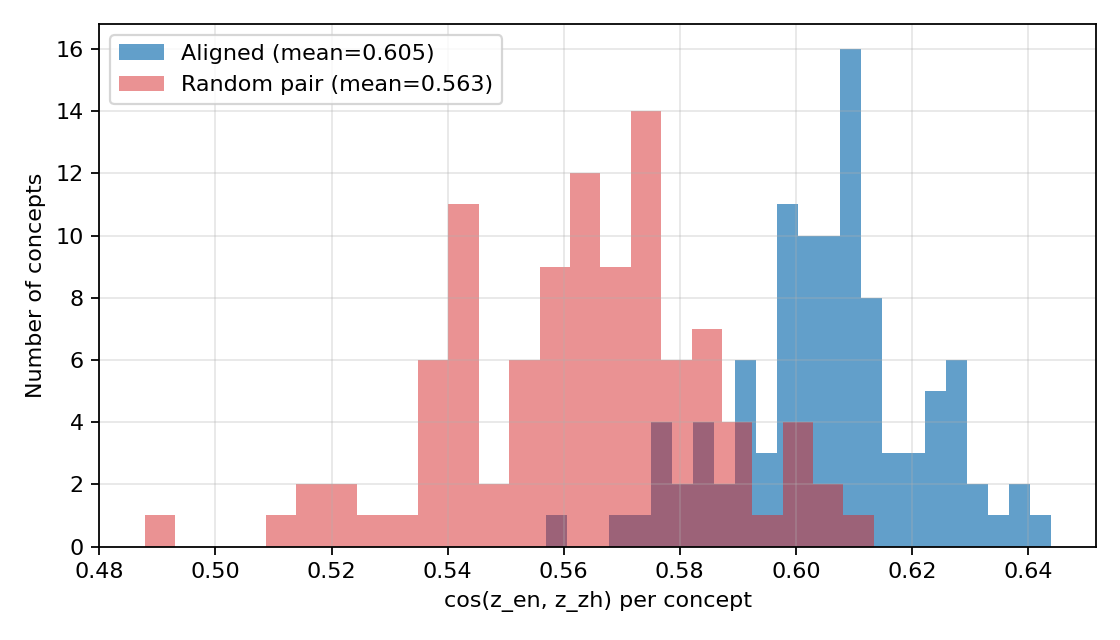
\includegraphics[width=0.72\linewidth]{figures/concept_consistency_hist}
\caption{Distribution of $\cos(Z_\text{en}[i], Z_\text{zh}[i])$ across
$N{=}102$ concepts (blue), against a permutation null (red) where Chinese
concepts are randomly re-assigned. The aligned distribution is reliably
right-shifted ($z=37.7$).}
\label{fig:concept_consistency}
\end{figure}

\subsection{RQ2: Feature typology}

Of $16{,}384$ dictionary atoms, $489$ are active on our probe set (others
are either dead or not exercised by these particular prompts; the SAE's
overall dead fraction on held-out data is only $0.3\%$, so most of the
remaining features simply do not fire on these short concept-centric
templates). Among the active features (Figure~\ref{fig:classification}):

\begin{itemize}
\item $\mathbf{62}$ \emph{Universal} features (cross-lingual corr.\ $\geq 0.5$).
\item $\mathbf{38}$ \emph{English-specific}.
\item $\mathbf{107}$ \emph{Chinese-specific}.
\item $\mathbf{1}$ \emph{Anti-aligned}.
\item $283$ \emph{Other} (weak alignment).
\end{itemize}

\begin{figure}[h]
\centering
\begin{subfigure}{0.46\linewidth}\centering
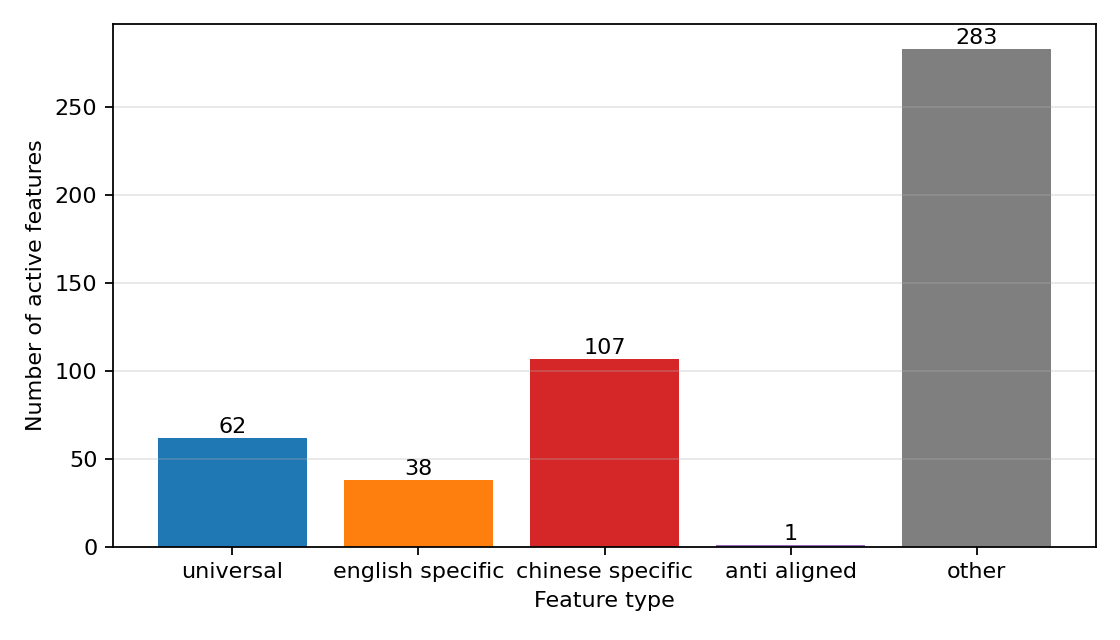
\includegraphics[width=\linewidth]{figures/feature_classification}
\caption{Counts.}
\end{subfigure}
\hfill
\begin{subfigure}{0.50\linewidth}\centering
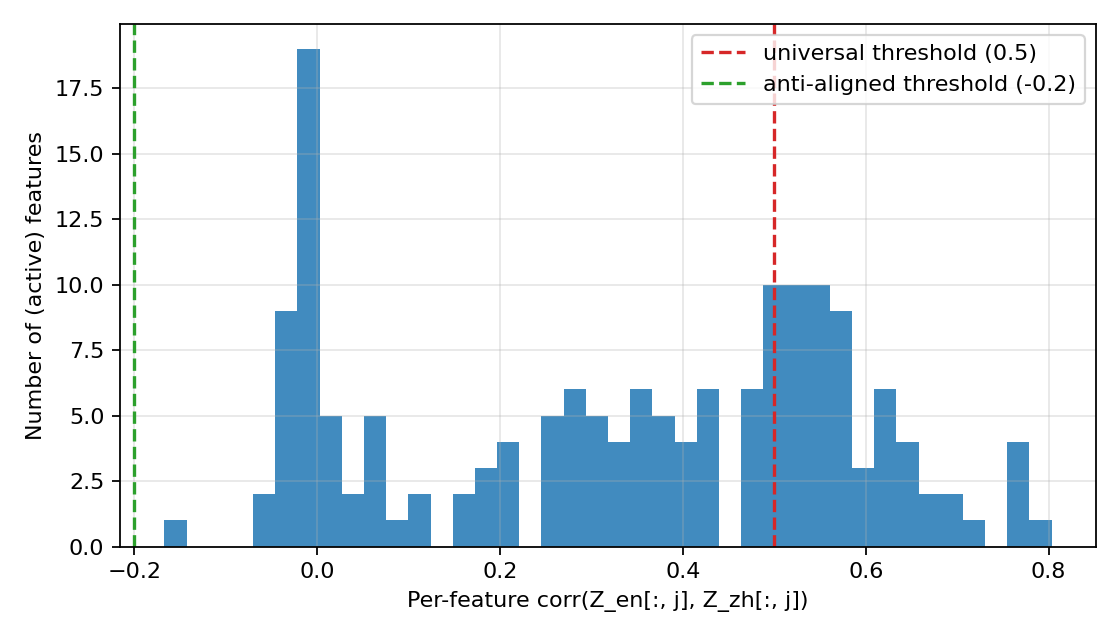
\includegraphics[width=\linewidth]{figures/feature_corr_hist}
\caption{Per-feature correlation distribution.}
\end{subfigure}
\caption{Feature typology on the 489 active features. The cross-lingual
correlation distribution is broad, with a substantial right tail
($\rho\geq 0.5$, 62 features) and almost no anti-aligned mass
($\rho\leq -0.2$, 1 feature).}
\label{fig:classification}
\end{figure}

Three observations:

(a) The marked imbalance Chinese-specific~($107$)~$>$~English-specific~($38$)
is consistent with Qwen's tokenisation: Chinese characters are often
single-token, so each Chinese token already carries substantial concept
mass and individual features can specialise to specific characters or
character bigrams, whereas English content words are typically split into
multiple subword tokens whose features may be more shared.

(b) The $62$ universal features are a small fraction of the dictionary,
but Figure~\ref{fig:classification}b shows a clear bimodal-like tail:
features either correlate weakly ($\rho$ near 0, reflecting noise / weak
template coupling) or correlate strongly ($\rho > 0.5$). There is essentially
no anti-aligned population (Figure~\ref{fig:classification}b).

(c) The scatter of $(\log v^\text{en}, \log v^\text{zh})$
(Figure~\ref{fig:feature_var_scatter}) shows three populations: a large mass
along the diagonal coloured red (high correlation, similar variance in both
languages), and two off-diagonal tails (language-specific features). Features
near the diagonal are typically those whose activation magnitude is
\emph{calibrated} across languages, an architectural prerequisite for being
``conceptual''.

\begin{figure}[h]
\centering
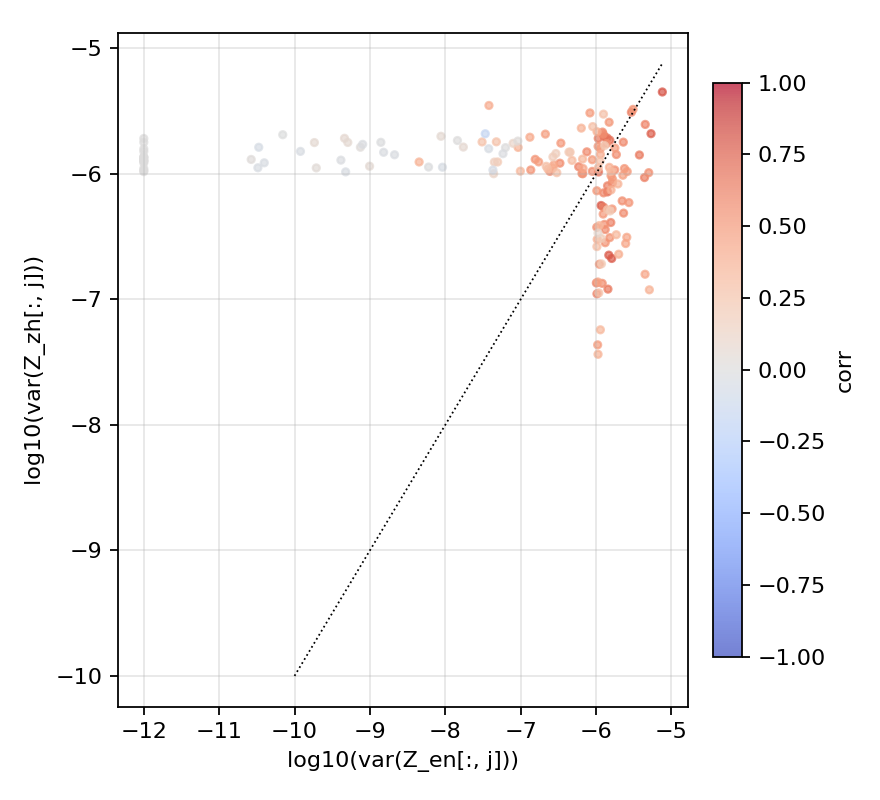
\includegraphics[width=0.55\linewidth]{figures/feature_var_scatter}
\caption{$\log_{10}$ per-feature variance, English vs.\ Chinese, coloured by
cross-lingual correlation. Diagonal mass is universal; off-diagonal tails are
language-specific.}
\label{fig:feature_var_scatter}
\end{figure}

\subsection{RQ3: Semantic type breakdown}

Per-category mean cosine and Jaccard@20 (top-features overlap) are shown in
Figure~\ref{fig:category_breakdown}. The most cross-lingually consistent
categories are \emph{tech}, \emph{action}, \emph{concrete-noun} and
\emph{animal} (cosine $\geq 0.609$); the least consistent are \emph{food}
($0.593$) and \emph{role} ($0.599$). The absolute gap is small ($0.025$) but
the ordering is intuitive: technological and action concepts (e.g.\
``algorithm''~/~``\zh{算法}''; ``running''~/~``\zh{跑步}'') tend to be modern, recently
borrowed, and culturally invariant, whereas food and social roles
(``rice''~/~``\zh{米饭}''; ``mother''~/~``\zh{母亲}'') carry culturally divergent
connotations and may activate different culture-specific features even when
the denotational content matches. Jaccard@20 follows a roughly similar but
noisier pattern, with \emph{country} and \emph{time} showing notably high
top-feature overlap, presumably because their denotational content is
strongly anchored to specific token identities (e.g.\ year markers, country
names) that the SAE assigns dedicated atoms to.

\begin{figure}[h]
\centering
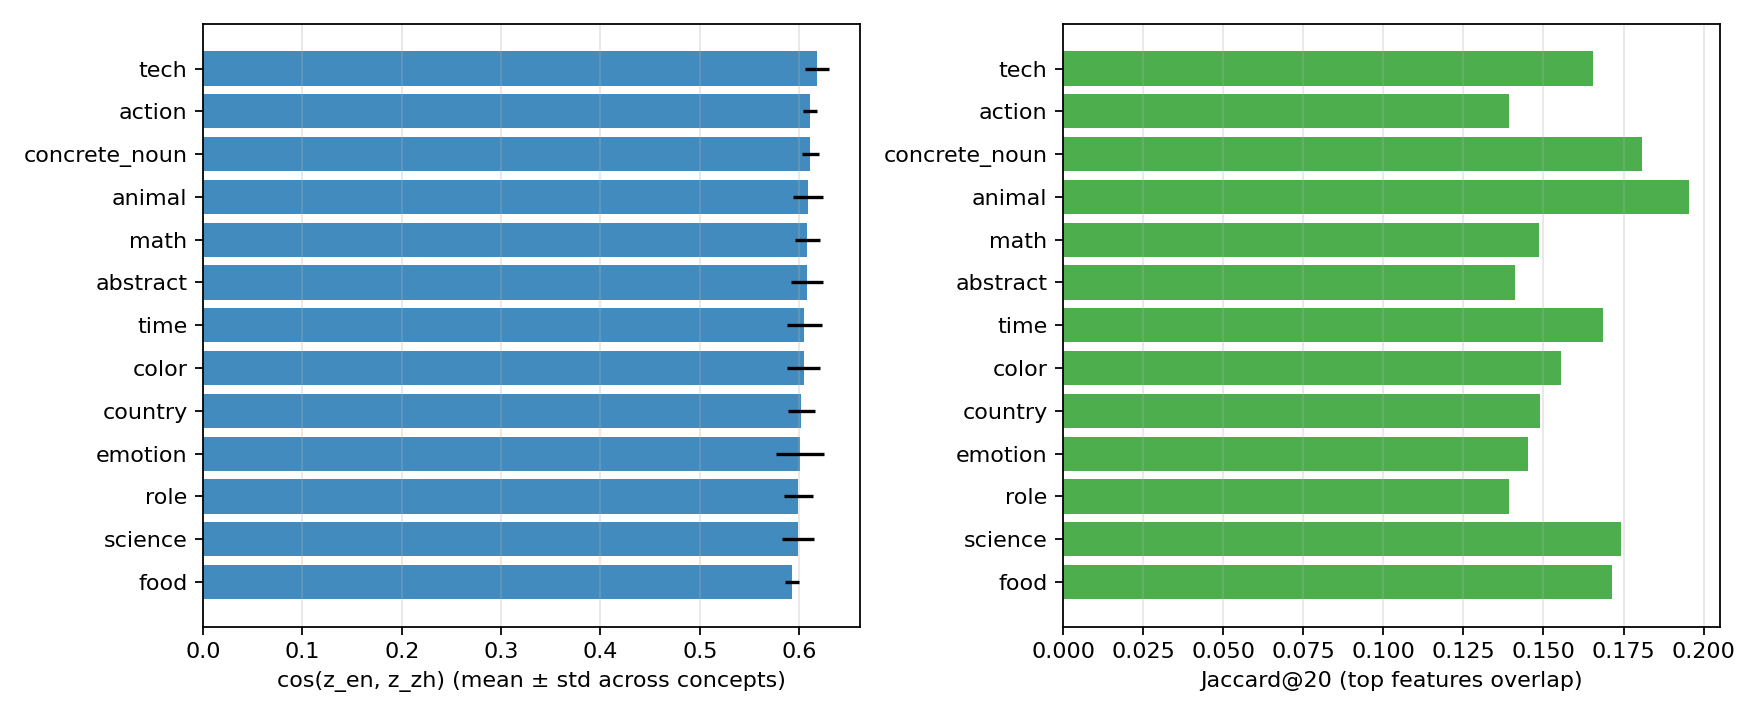
\includegraphics[width=0.93\linewidth]{figures/category_breakdown}
\caption{Per-category cross-lingual cosine (left, mean$\pm$std) and Jaccard
of the top-20 features (right), sorted by cosine.}
\label{fig:category_breakdown}
\end{figure}

\subsection{Logit-lens readout}

Decoding the top-20 unembedding-projected tokens for the top-30 features in
each typology class (Figure~\ref{fig:lens}) shows that all three typology
classes include a non-negligible Chinese token share, including features
nominally tagged as \emph{English-specific}. We interpret this as a known
limitation of mid-layer logit-lens \cite{nostalgebraist2020interpreting}:
at layer~12 of 24, the residual stream has not yet been ``finalised'', and
projecting through the final norm + unembedding is only an
approximation. Still, qualitative spot-checks of the top universal features
(Table~\ref{tab:lens_examples}) reveal occasional cross-lingual content
binding---e.g.\ feature $\#10837$ surfaces (\zh{席, 比例为}, Share, \zh{占到}, inte),
a coherent ``proportional share'' cluster mixing Chinese and English tokens.

\begin{figure}[h]
\centering
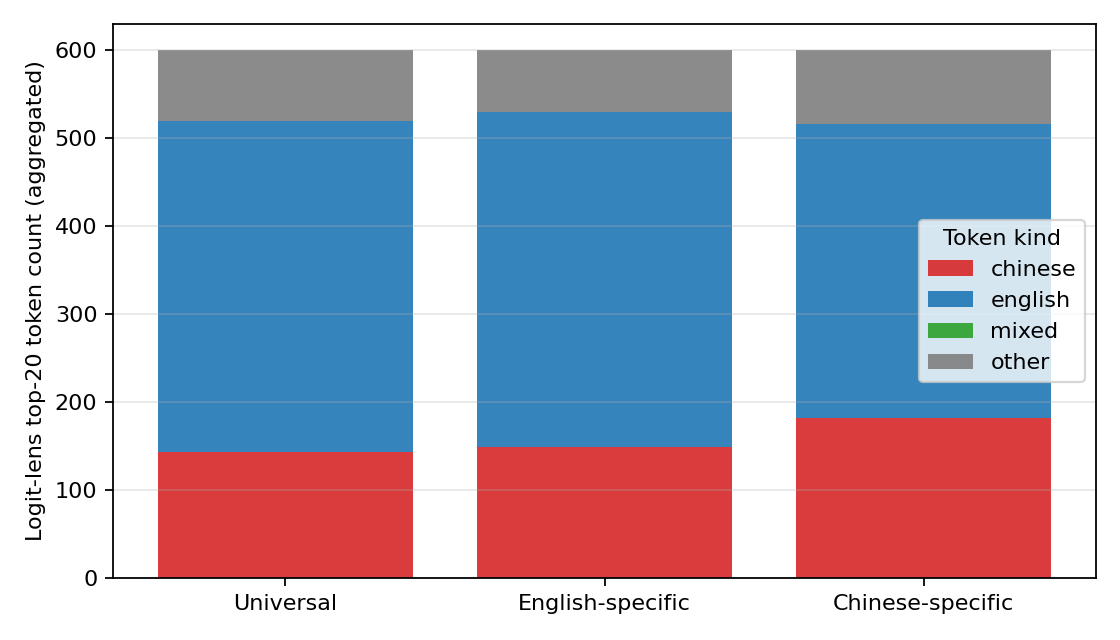
\includegraphics[width=0.66\linewidth]{figures/lens_token_kind}
\caption{Aggregated count of the top-20 logit-lens tokens (over top-30
features per class) by token kind. Universal features show a 24\% Chinese /
63\% English mixture, marginally more bilingual than the language-specific
classes.}
\label{fig:lens}
\end{figure}

\begin{table}[h]
\centering\small
\begin{CJK*}{UTF8}{gbsn}
\begin{tabular}{rcl}
\toprule
Feature & $\rho_j$ & Top logit-lens tokens (truncated) \\
\midrule
$10837$ & $0.803$ & 席 \,$|$\, 比例为 \,$|$\, onom \,$|$\, Share \,$|$\, 占到 \,$|$\, inte \\
$13346$ & $0.764$ & il \,$|$\, 名学生 \,$|$\, wad \,$|$\, signature \,$|$\, 格尔 \,$|$\, G \\
$5323$ & $0.729$ & ereien \,$|$\, rasında \,$|$\, 理事长 \,$|$\, Deportes \,$|$\, 海默 \\
$1269$ & $0.644$ & 既 \,$|$\, asikan \,$|$\, 谣言 \,$|$\, pre \,$|$\, 描述 \\
$10416$ & $0.649$ & ement \,$|$\, acid \,$|$\, ure \,$|$\, opl \,$|$\, U \,$|$\, EMENT \\
\bottomrule
\end{tabular}
\end{CJK*}
\caption{Top universal features by cross-lingual $\rho_j$, with their
logit-lens top tokens. Notable: $\#10837$ mixes English and Chinese
``proportion'' words.}
\label{tab:lens_examples}
\end{table}

\subsection{RQ4: Cross-lingual steering}

We steer the model along the top-3 universal-feature decoder directions
($j\in\{10837, 13346, 5323\}$), at coefficients
$\alpha\in\{0, 4, 12, 30\}$, on three English and three Chinese ``neutral''
continuation prompts (Figure~\ref{fig:steering_kl}). KL from baseline grows
monotonically with $\alpha$, with English and Chinese curves tracking each
other closely for each feature. For $j{=}10837$, $\alpha{=}4$ already
induces KL of $1.0$--$4.6$ nats; for $j{=}13346$ and $\alpha{=}4$ KL is in
the $0.6$--$1.9$ range. Crucially the cross-lingual ratio
$\mathrm{KL}_\text{zh} / \mathrm{KL}_\text{en}$ remains within
$0.6$--$2.0$ across alphas, indicating broadly comparable effect sizes.

Qualitatively, modest steering ($\alpha{=}4$) preserves fluency and shifts
content in similar ways across languages: e.g.\ $\#5323$ at $\alpha{=}4$
induces repetition / iteration patterns in both English
(``\emph{let's say, let's say, let's say\ldots}'') and Chinese
(``\zh{\emph{比如，比如，比如，继续继续，继续，继续}}\ldots'').
Stronger steering ($\alpha\geq 12$) collapses generation to repetitive
nonce-token streams (e.g.\ ``\emph{iteln iteln ving iteln}''), indicating
that the SAE features remain \emph{polysemantic} at this small scale and
that pushing along a feature direction at large magnitude leaves the
trained manifold; this is consistent with reports for smaller SAEs
\cite{bricken2023monosemanticity}.

\begin{figure}[h]
\centering
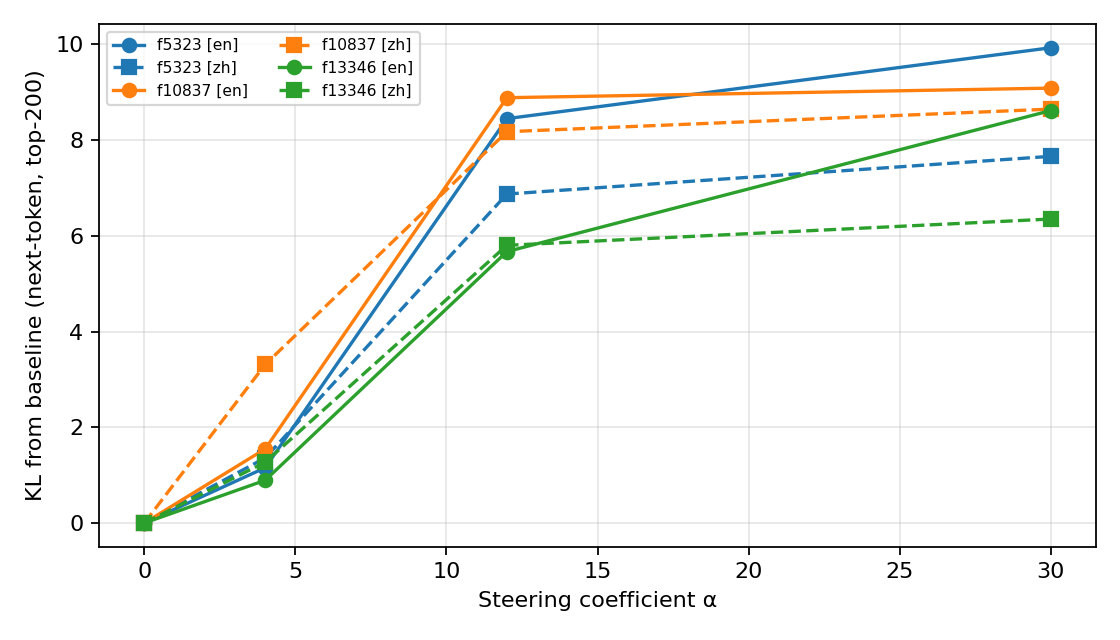
\includegraphics[width=0.72\linewidth]{figures/steering_kl_vs_alpha}
\caption{Next-token KL divergence (vs.\ unsteered baseline, top-200) as a
function of steering coefficient $\alpha$ for the top-3 universal features.
Solid lines: English prompts. Dashed lines: Chinese prompts. The two
languages track each other closely for each feature.}
\label{fig:steering_kl}
\end{figure}

\section{Discussion}

\paragraph{What we (carefully) conclude.}
A small multilingual model does host a population of mid-layer SAE features
whose activations are reliably synchronised between English and Chinese
expressions of the same concept, and steering along such features induces
comparable next-token-distribution shifts across languages. These features
are a minority among active atoms (62 of 489 in our probe), consistent with
the idea that mid-layer representations are largely surface-form and
tokeniser-driven, with conceptual content being a real but second-order
component.

\paragraph{What we cannot conclude.}
We do not claim that Qwen3.5 has a single language-neutral semantic space.
The mean cross-lingual cosine of $0.605$ is well below 1, and is only
$\sim 0.04$ above an aggressive permutation baseline. The category gap
(tech $-$ food $=0.025$) is statistically detectable but small. At the
feature level, even our top-$\rho$ universal features look polysemantic
under logit-lens inspection. We \emph{do not} claim cross-lingual
monosemanticity at this scale.

\paragraph{Why might the signal be small?}
We see three plausible contributors. (1) \emph{Model scale and SAE width.}
With $d_\text{sae}/d_\text{in}=16$ in a 0.8B model, the dictionary may simply
be too coarse to disentangle concept from language. Larger expansions
(64$\times$, 128$\times$) and larger backbones in
\cite{templeton2024scalingmonosemanticity} report much cleaner universal
features. (2) \emph{Tokenisation asymmetry.} Chinese tokens are dense (one
char $\approx$ one token), English tokens are sparse (multi-piece). This
biases mid-layer features toward different granularities in the two languages.
(3) \emph{Layer choice.} Layer~12 is the middle of a 24-layer model;
\cite{wendler2024llamasenglish} suggests deeper layers carry more
language-agnostic semantics in Llama-2. A multi-layer SAE sweep would likely
shift the proportion of universal features.

\paragraph{Implications for SAE-based interpretability of small multilingual models.}
We see two practical lessons. First, when interpreting features in a
multilingual SAE, automatic interpretation pipelines that rely on
English-only datasets risk severely undercounting genuine cross-lingual
features and miscalibrating estimates of feature monosemanticity.
Second, ``feature ablation / steering'' studies on multilingual models
should test both the source language and at least one other to verify the
intended causal effect is not language-specific.

\section{Limitations}

\begin{itemize}
\item \textbf{Probe scale.} 102 concepts in 5 templates is small. Replication
on larger parallel corpora (e.g.\ OPUS, FLORES) would tighten estimates.
\item \textbf{Single hook layer.} We probe layer~12 only. A layer sweep is a
natural follow-up.
\item \textbf{Single SAE variant.} We use Top-K \cite{gao2024scalingsae}.
JumpReLU \cite{rajamanoharan2024jumprelu} and Matryoshka SAEs may localise
universality differently.
\item \textbf{Token-averaging.} We average $z$ over all non-pad tokens,
which dilutes the concept signal with template tokens. A position-aware
analysis isolating the concept-token positions would likely sharpen the
effect.
\item \textbf{Logit-lens at mid-layer.} Our token-kind readout is only
suggestive; activation-maximising prompts or causal-tracing studies would be
more reliable.
\item \textbf{Steering qualitative-only.} Beyond KL we did not yet build an
automatic classifier of ``did the concept appear in the continuation''; a
benchmark like \cite{templeton2024scalingmonosemanticity}'s qualitative grid
would strengthen RQ4.
\end{itemize}

\section{Conclusion}

We presented a simple SAE-based psycholinguistic probe for a small
multilingual language model. Cross-lingual concept consistency is real and
statistically robust at the population level ($z=37.7$ above a permutation
baseline), and at the feature level a small but well-defined universal
population can be isolated and causally steered. The effect's modest
magnitude---a $\sim 4\%$ cosine boost over permutation, $13\%$ of active
features qualifying as universal, and $\sim 0.025$ category-level
differentiation---reminds us that mid-layer representations in sub-1B
multilingual models are mostly surface-form, with semantics as a real but
second-order signal. We release all code, configurations, the parallel
concept probe set, and figures to support replication and extension.

\paragraph{Reproducibility.}
All experiments use a single RTX~5070~Ti Laptop. Training, evaluation,
probe data and analysis scripts are under
\texttt{src/}, \texttt{configs/}, \texttt{data/psych/} and
\texttt{results/topk\_l12\_local\_2/}, \texttt{results/crosslingual\_3/}.
Conda environment specification and exact run commands are documented in
\texttt{GUIDE/} and \texttt{\_memory/}.

\bibliographystyle{plain}
\bibliography{refs}

\end{document}
